\section{RL For Navigation}\label{sec:navigation}

\subsection{Problem Formulation}\label{subsec:problem-formulation}

We address the VSN problem by using Reinforcement Learning (RL).
Thus, navigation can be described as a partially observable Markov decision process (POMDP), in which the agent, \ie, a robot, navigates through an environment and tries to reach a determined object.
This problem is known in the literature as the ObjectNav task~\cite{batra2020}.

Formally, given an initial observation distribution $p_0$, for the step $t$ the agent receives an observation $o_t \sim p_0(o)$ based on state $s_t$, which in our case is just an RGB image of what the robot observes.
The agent takes action $a_t$, obtains reward $r_t$ from the environment and receives a new observation $o_{t+1} = \mathcal{T} (o_{t+1}|o_t, a_t)$, where $\mathcal{T}$ is the transition function.
An episode is a sequence of $\left(o_t, a_t, r_t\right)$ tuples that form a trajectory.
The episode ends when the agent reaches the goal or the maximum number of steps ($H$).
An episode is considered a success if the agent reaches the goal within the step horizon $H$.

The goal is to find an optimal policy $\pi^*$ that maximizes the cumulative reward over an episode.
This policy maps observations to a probability distribution over actions that is specified as follows,
\begin{equation}
    \label{eq:op_policy}
    \pi^*=\argmax\limits_\pi\mathbb{E}_{\mathcal{T}\sim\pi}[R_H],
\end{equation}
where $R_H=\sum_{t=1}^H \gamma^{t-1}r_t$ is the return, \ie the cumulative reward over an episode, and $\gamma$ is a discount factor.
In navigation tasks, neural networks with parameters $\theta$ are often used to parameterize the policy $\pi_\theta$.

\subsection{Visual Semantic Navigation}\label{subsec:visual-semantic-navigation}

Learning to navigate in a given environment is a challenging task.
First, the reward signal coming from the environment is usually sparse~\cite{sutton2018, pathak2017}.
These sparse rewards lead to a quite difficult training process.
%Second, the agent has to balance an exploration of the environment to obtain experience and the exploitation of the previous experience in order to obtain successful episodes~\cite{sutton2018, mnih2013}.
Second, we need to find a balance between the exploration and exploitation of the environment to achieve successful experiences that drive the agent's learning process~\cite{sutton2018, mnih2013}.
Finally, the agent architecture has a direct impact on how it learns.
State-of-the-art approaches use a feature extractor followed by recurrent units to process temporal information coming from the images.
%For navigation tasks, a common agent architecture consists of a CNN feature extractor and an RNN that outputs the action distribution.

\textbf{Sparse rewards and long horizon.}
%In visual navigation, sparse rewards are a common issue due to the nature of the task, \ie reaching a specific target in an environment.
Sparse rewards are a common issue due to the nature of the navigation tasks, \ie reaching a specific target in an environment.
The most straightforward way to define a reward in navigation problems is to let the environment provide a fixed amount when the agent reaches the goal.
This means the agent has to face an environment in which:
1) in the best case, most of the reward signal is zero except for the step in which the agent reaches the goal and obtains a certain amount of reward;
and 2) if the agent does not reach the target it does not receive any reward.
This situation worsens with large temporal horizons, because the more steps, the higher the sparsity of the reward is.

To mitigate the sparse reward problem, we use a technique called reward shaping.
It consists in modifying the original reward signal via incorporating domain knowledge.
For navigation, we leverage on the \textit{distance reward}~\cite{wijmans2020}, defined as:
\begin{equation}
    \label{eq:rew_shaping}
    r_t = -d(s_t, target) + d(s_{t+1}, target) - r_s + r_T,
\end{equation}
where $d(s_t, target)$ computes the geodesic distance between agent's position at state $s_t$ and $target$'s position.
$r_T$ is the \textit{terminal reward}, a fixed amount given only when the agent reaches the target and $r_s=0.01$ is the \textit{slack reward}, also a fixed amount that penalizes each step.
The goal of the \textit{distance reward} function is to give a constant reward signal to the agent that increases as the agent approaches the target.
In section~\ref{subsec:miniworld-maze-results} we compare the \textit{distance reward} against what is usually referred to as the \textit{navigation reward}, which consists only of the slack reward and the terminal reward $r_t = -r_s + r_T$.

\textbf{Exploration vs. Exploitation.}
%As we have mentioned, in a navigation problem, our agent must explore the environment in order to find the trajectories that return the maximum amount of reward without surpassing the temporal horizon of $H$ steps.
%This exploration has to be balanced with respect to the exploitation process, in which the agent uses the previous knowledge to actively select the best actions to obtain the shortest successful episodes.
As we have mentioned, the exploration process has to be managed to encourage the agent to choose actions that it would not otherwise select.
To address this issue, we leverage the technique known as $\epsilon\text{-}greedy$~\cite{mnih2013}.
This solution \emph{controls} the action that is being selected by the agent, usually during the learning process.
Given an $\epsilon \in [0, 1]$, an action $a_t$ is selected as
\begin{equation}
    \label{eq:eps-greedy}
    a_t = \begin{cases}
              \argmax\pi_\theta & \mbox{with probability 1-$\epsilon$,}     \\
              rand(a) \in \mathcal{A} & \mbox{with probability $\epsilon$,} \\
    \end{cases}
\end{equation}
where $\mathcal{A}$ defines the action space.
Typically, $\epsilon$ starts at $1$ and it decays with the iterations.
In the beginning of the learning process, \ie when $\epsilon$ is high, random actions are sampled more often, encouraging the agent to explore the environment.
As the training process advances, lower $\epsilon$ values permit the agent to exploit the model knowledge to select the best action.
This introduces a balance between exploration and exploitation.

\textbf{Agent architecture.} We encode the agent as a parameterized model consisting in a CLIP~\cite{khandelwal2022} visual encoder connected to two actor-critic LSTMs that output a discrete distribution over the action space and the value, respectively.
A diagram of the implemented agent can be found in figure~\ref{fig:network_clip_diagram}.
To train the models, we use Proximal Policy Optimization (PPO)~\cite{schulman2017}, an on-policy RL algorithm.

\begin{figure}[t]
    \centering
    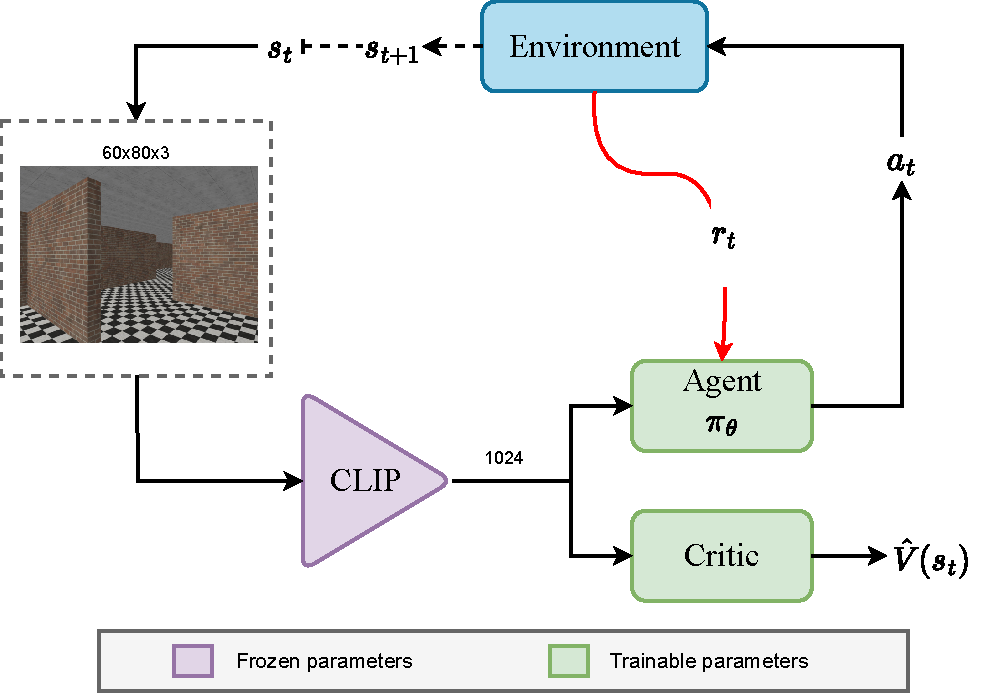
\includegraphics[width=0.8\linewidth]{figures/understanding_vsn/network_clip_diagram}
    \caption{\textbf{Model diagram}. This figure contains a high level representation of the model used: a visual encoder followed by an actor-critic module encoded by LSTMs. The visual encoder is frozen and we only train the actor-critic module.}
    \label{fig:network_clip_diagram}
\end{figure}
